\documentclass[12pt, a4paper]{report}
\usepackage[]{geometry, scrlayer-scrpage, sectsty, amsmath, amssymb, scrlayer-scrpage, graphicx, listings, xcolor}
\sectionfont{\huge}
\usepackage[onehalfspacing]{setspace}
\geometry{headheight=7.5cm, headsep=1cm}
\geometry{footskip=4.0cm}
\pagestyle{scrheadings}
\ihead{Robotic Games \\\today}
\ohead{Enrico Kaack, Robin Fleige, Laura Nell}
\cfoot{\pagemark}

\definecolor{codegreen}{rgb}{0,0.6,0}
\definecolor{codegray}{rgb}{0.5,0.5,0.5}
\definecolor{codepurple}{rgb}{0.58,0,0.82}
\definecolor{backcolour}{rgb}{0.95,0.95,0.92}

\lstdefinestyle{mystyle}{backgroundcolor=\color{backcolour},   
    commentstyle=\color{codegreen},
    keywordstyle=\color{magenta},
    numberstyle=\tiny\color{codegray},
    stringstyle=\color{codepurple},
    basicstyle=\ttfamily\footnotesize,
    breakatwhitespace=false,         
    breaklines=true,                 
    captionpos=b,                    
    keepspaces=true,                 
    numbers=left,                    
    numbersep=5pt}
    
\lstset{style=mystyle, language=Python}



\begin{document}

\begin{titlepage}

        \centering
        \vspace{1cm}
        {\scshape\Large Robotic Games WS19/20 \par}
        \vspace{1.5cm}
        {\huge\bfseries Zwischenbericht \par}
        \vspace{2cm}
        {\Large\itshape Enrico Kaack, Robin Fleige, Laura Nell \par}

    
        \vfill
    
    % Bottom of the page
        {\large \today\par}
    \end{titlepage}
\newpage    

\pagenumbering{arabic}
\onehalfspacing


\chapter{Implementierung}

\section{Collision avoidance}
Um die Kollisionsvermeidung zu verwirklichen, wird die Momentangeschwindigkeit des Roboters durch einen Subscriber ausgelesen. Zusätzlich sind auf die gleiche Weise die Messwerte der Soanrsensoren in Form von Abständen zum nächsten Hindernis bekannt.
Für die Kollisionsvermeidung wird ein Kraftansatz gewählt, bei welchem die Kraft, welche auf den Roboter durch ein sich näherndes Hindernis ausgeübt wird, die Änderung der Linear- und Winkelgeschwindigkeit bestimmt. Dies ist in der folgenden Funktion \textit{calculate\_force(self, sonar\_angles, sonar\_ranges)} verwirklicht. Dabie handelt es sich bei sonar\_angles um die Winkel, in welchen die Sonarsensoren vom Roboter abstrahlen und bei sonar\_ranges um den jeweils zurückgegebenen Abstand.
\begin{lstlisting}
def calculate_force(self, sonar_angles, sonar_ranges):
  sum = np.zeros(2)

  for i, sonar_range in enumerate(sonar_ranges):
      if sonar_range == 0.0:
          rospy.logerr('Catched Zero')
          sonar_range = 1e-12
      vec = np.array([1/sonar_range * np.cos(sonar_angles[i]), 1/sonar_range * np.sin(sonar_angles[i])])
      sum += vec
          
  sum *= (-1)
  sum_dist = np.linalg.norm(sum)
       
  if sum_dist < 10.0:
      return np.zeros(2)

  phi = -np.arctan2(sum[1], sum[0])
  force = np.zeros(2)
  force[0] = np.clip(-sum[0] / 20, 0, 1)
  force[1] = np.clip(phi, -np.pi/2, np.pi/2)

  if -force[1] == self.last_angle:
      force[1] = self.last_angle

  self.last_angle = force[1]
  return force
  
\end{lstlisting}
Um die auf den gesamten Roboter wirkende \''Kraft\'' zu bestimmen, wird die Resultierende aus allen von den Sonarsensoren aufgezeichneten Abständen bestimmt. Dazu werden diese in der for-Schleife ab Zeile 4 zunächst in ihre x- und y-Komponenten unterteilt und diese im Array \textit{sum} aufsummiert. Da die \''Kraft\'' entgegen des Roboters wirken soll, wird dieses negiert und anschließend der auf den Roboter wirkende Vektor mithilfe der Funktion \textit{numpy.linalg.norm()} berechnet.\\
Sollte der resultierende Abstand zu einem Hindernis noch größer als 10m sein, wird der Fahrtweg des Roboters nicht verändert, es wird ein Nullarray zurückgegeben $($Zeile 14f.$)$.\\
In jedem anderen Fall wird das Array \textit{force[ ]} erstellt und zurückgegeben, wobei \textit{force[0]} die Änderung der Linearbeschleunigung beinhaltet und \textit{force[1]} die Änderung der Winkelbeschleunigung. Die Berechnung der Änderung der Linear- und Winkelbeschleunigung erfolgt mithilfe der Funktion \textit{numpy.clip(a, a\_min, a\_max)}, welche den Wert von a auf das Intervall $[$a\_min, a\_max$]$ beschränkt. Liegt der Wert a unterhalb a\_min, wird a\_min zurückgegeben, liegt a überhalb a\_max, wird a\_max zurückgegeben. \\
Da die Änderung der Lineargeschwindigkeit an den Roboter in der Form 1 - $\Delta$x übermittelt wird, wird der x-Anteil des resultierenden Vektors / 20 hierfür auf das Intervall $[$0,1$]$ begrenzt, da der Roboter nicht rückwärts fahren soll $($negative Linearbeschleunigung$)$ $($Zeile 19$)$. Damit wird die Lineargeschwindigkeit nicht geändert, wenn der Wert x/20 oberhalb von 1 liegt, also der Abstand des Roboters zum Hindernis in x-Richtung noch groß genug ist, und maximal geändert, sollte der Wert negativ sein. Dieser Fall sollte allerdings nie eintreten, da dies bedeuten würde, dass der Roboter bereits an/hinter der Wand steht.\\
Die Änderung der Winkelbeschleunigung wird über den negativen arctan2 des resultierenden Vektors, begrenzt auf $[$-$\pi$/2, $\pi$/2$]$, bestimmt $($Zeile 20$)$. Dabei sind die Maximalwerte so gewählt, dass sich der Roboter in einem Schritt nicht zu viel dreht, sondern dies auf mehrere Schritte aufgeteilt wird.\\
Sollte der Roboter genau senkrecht auf eine Ecke zufahren, kann der Fall auftreten, dass die resultierende \''Kraft\'' genau senkrecht auf den Roboter wirkt bzw. dadurch die Änderung der Winkelbeschleunigung zwischen beiden Seiten alterniert, sodass der Roboter sich nicht befreien kann. Dies wird abgefangen, indem die Änderung der Winkelbeschleunigung in diesem Fall auf den positiven Fall festgesetzt wird $($Zeile  22f.$)$.
Die zurückgegebenen Werte werden dem Roboter mithilfe eines Publishers übermittelt.\\


Die Funktionalität des implementierten Programms wird anhand der zur Verfügung gestellten Funktion \textit{create\_visualisation} geprüft und visualisiert. In den folgenden Abbildung sind dessen Ergebnisse gegenübergestellt.\\\\\\\begin{centering}
Visualisieriung Welt 1\\
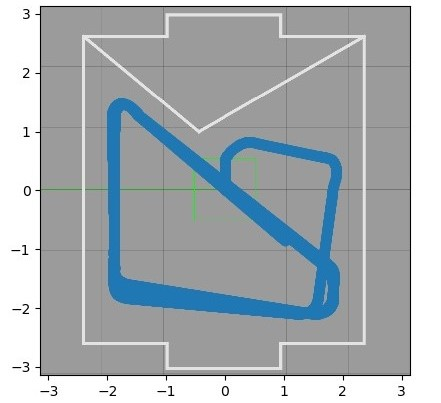
\includegraphics[width=290pt]{roboter_pfad1.jpg}\newpage
Visualisieriung Welt 2\\
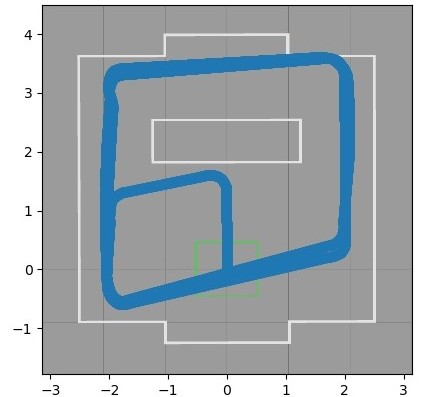
\includegraphics[width=290pt]{roboter_pfad2.jpg}\\
~\\
Visualisieriung Welt 3\\
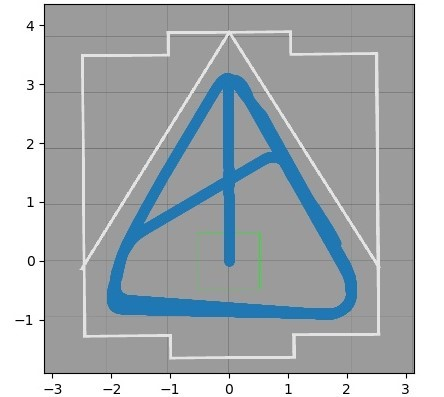
\includegraphics[width=290pt]{roboter_pfad3.jpg}\newpage
Visualisieriung Welt 4\\
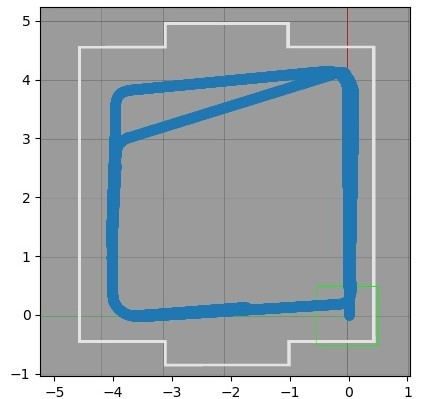
\includegraphics[width=290pt]{roboter_pfad4.jpg}\\
~\\
Visualisieriung Welt 5\\
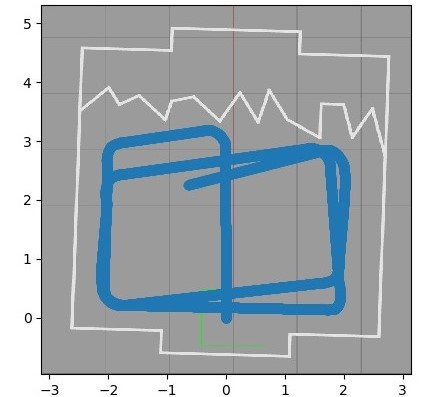
\includegraphics[width=290pt]{roboter_pfad5.jpg}\\
\end{centering}


\textcolor{red}{Diskussion $\rightarrow$ Verbesserungen?}
\newline

\section{Homing}
\begin{lstlisting}
rospy.Subscriber("dead_reckoning", Pose, self.callback)
\end{lstlisting}

\begin{lstlisting}
def callback(self, pos):
  self.orientation[0] = pos.orientation.z
  self.position[0] = pos.position.x
  self.position[1] = pos.position.y
\end{lstlisting}

\begin{lstlisting}
def closed_loop(position,orientation,target):
  output=Twist()

  target_rel_x = target[0] - position[0]
  target_rel_y = target[1] - position[1]

  dir_x = np.cos(orientation[0]-np.pi/2)*target_rel_x + np.sin(orientation[0]-np.pi/2)*target_rel_y
  dir_y = np.cos(orientation[0]-np.pi/2)*target_rel_y - np.sin(orientation[0]-np.pi/2)*target_rel_x

  if np.abs(np.arctan2(dir_x, dir_y)) < np.pi/4 and dir_x*dir_x+dir_y*dir_y > 0.01:
      output.linear.x = 0.5
  else:
      output.linear.x = 0
  if np.abs(np.arctan2(dir_x,dir_y)) > np.pi/30:
      output.angular.z = np.arctan2(dir_x, dir_y)/3

  return output
  
\end{lstlisting}

\section{Free Space}

Das Free Space Verhalten soll dafür sorgen, dass der Roboter in Richtung der freien Fläche im Raum fährt. Die zur Verfügung stehenden Informationen beschränken sich dabei auf die vorhandenen acht Ultraschall Sensoren und deren Entfernungsmessung.
\\
Der Algorithmus prüft, ob die größte Entfernung links oder rechts der Hauptachse gemessen wurde und dreht den Roboter entsprechend nach rechts oder links mit einer konstanten Drehrate. 
\\
Bei diesem Ansatz werden an zwei Stellen Probleme erwartet. Zum einen wird der Sensor mit der maximalen Entfernung zur Bestimmung der Drehrichtung benutzt. Wenn dieser Sensor allerdings einen Gang misst, der vom Roboter weg verläuft, würde sich der Roboter in diese Richtung orientieren. Dieses Verhalten wäre dementsprechend falsch, da der Gang nicht der freien Fläche entspricht. Um dem entgegen zu wirken, könnte man die Sensorwerte von jeweils der rechten und linken Seite mitteln und darauf basierend die Richtungsentscheidung treffen. Im späteren Schritt der Fusion wird der Free Space Teil allerdings nur eine untergeordnete Rolle spielen, sodass dieses Problem nicht in dieser Form auftritt.\\
Eine zweite Schwäche liegt darin, dass eine konstante Drehrate in die jeweilige Richtung gesetzt wird. Eine Auswirkung hiervon wäre, dass bei zu hoher Geschiwndigkeit der Roboter gegen ein Hindernis fahren könnte, da die konstante Drehrate nicht auf die Lineargeschwindigkeit angepasst ist und der Kurvenradius demnach größer wird. Eine Lineargeschwindigkeit abhängig von der Entfernung des Sensors mit der niedrigsten Entfernung würde dies beheben. Sollte in der Fusion dies zu einem Problem führen, wird diese Idee entsprechend aufgegriffen. Da allerdings die Kollisionsvermeidung eine höhere Gewichtung in der Nähe einer Wand erhalten wird, sollte dies nicht zu einem Problem führen.


\section*{Verhaltensfusion}




\end{document}











